\section{Determination of defects}
\mn{appendix,obligation=normative}
\label{AnnexA}

\subsection{Principle}

Extraneous matter, broken kernels, damaged kernels and other kinds of rice are separated manually according to the following types: husked rice, milled rice, husked parboiled rice and milled parboiled rice. Each type is then weighed.

\subsection{Apparatus}

The usual laboratory apparatus and, in particular, the following.

\subsubsection{Sample divider,}
\mn{\%inline-header}
\label{AnnexA-2-1}

consisting of a conical sample divider or multiple-slot sample divider with a distribution system, e.g. "Split-it-right" sample divider, such as that shown in \ref{figureA-1}.

\subsubsection{Sieve,}
\mn{\%inline-header}

with round perforations of diameter 1,4 mm.

\subsubsection{Tweezers.}
\mn{\%inline-header}

\subsubsection{Scalpel.}
\mn{\%inline-header}

\subsubsection{Paintbrush.}
\mn{\%inline-header}

\label{AnnexA-2-6}
\subsubsection{Steel bowls,}
\mn{\%inline-header}

of diameter 100 mm $\pm$ 5 mm; seven per test sample.

\subsubsection{Balance,}
\mn{\%inline-header}

which can be read to the nearest 0,01 g.

\subsection{Sampling}

See \ref{clause5}.

\subsection{Procedure}

\label{AnnexA-4-1}
\subsubsection{Preparation of test sample}

Carefully mix the laboratory sample to make it as uniform as possible, then proceed to reduce it, using a divider (\ref{AnnexA-2-1}), until a quantity of about 30 g is obtained.

All parts of kernels which get stuck in the perforations of a sieve should be considered to be retained by the sieve.

\begin{figure}
  \label{figureA-1}
  \caption{Split-it-right sample divider}
  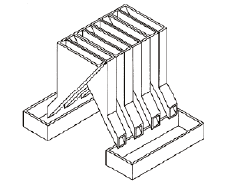
\includegraphics{images/a1.png}
\end{figure}

\subsection{Determination}

Weigh, to the nearest 0,1 g, one of the test samples obtained in accordance with \ref{AnnexA-4-1} and separate the different defects into the bowls (\ref{AnnexA-2-6}). When a kernel has several defects, classify it in the defect category for which the maximum permissible value is the lowest (see \ref{table1}).

Weigh, to the nearest 0,01 g, the fractions so obtained.

\subsection{Calculation}

Express the mass fraction of each defect using \ref{formulaA-1}:

% [[formulaA-1,A.1]]
\begin{equation}\label{formulaA-1}
  w = (m_D) / (m_s)
\end{equation}

where

\begin{description}
  \item[$w$] is the mass fraction of grains with a particular defect in the test sample;
  \item[$m_D$] is the mass, in grams, of grains with that defect;
  \item[$m_S$] is the mass, in grams, of the test sample.
\end{description}

\subsection{Test report}

Report the results as specified in \ref{clause7}.
